% Options for packages loaded elsewhere
\PassOptionsToPackage{unicode}{hyperref}
\PassOptionsToPackage{hyphens}{url}
\PassOptionsToPackage{dvipsnames,svgnames,x11names}{xcolor}
%
\documentclass[
  letterpaper,
  DIV=11,
  numbers=noendperiod]{scrartcl}

\usepackage{amsmath,amssymb}
\usepackage{lmodern}
\usepackage{iftex}
\ifPDFTeX
  \usepackage[T1]{fontenc}
  \usepackage[utf8]{inputenc}
  \usepackage{textcomp} % provide euro and other symbols
\else % if luatex or xetex
  \usepackage{unicode-math}
  \defaultfontfeatures{Scale=MatchLowercase}
  \defaultfontfeatures[\rmfamily]{Ligatures=TeX,Scale=1}
\fi
% Use upquote if available, for straight quotes in verbatim environments
\IfFileExists{upquote.sty}{\usepackage{upquote}}{}
\IfFileExists{microtype.sty}{% use microtype if available
  \usepackage[]{microtype}
  \UseMicrotypeSet[protrusion]{basicmath} % disable protrusion for tt fonts
}{}
\makeatletter
\@ifundefined{KOMAClassName}{% if non-KOMA class
  \IfFileExists{parskip.sty}{%
    \usepackage{parskip}
  }{% else
    \setlength{\parindent}{0pt}
    \setlength{\parskip}{6pt plus 2pt minus 1pt}}
}{% if KOMA class
  \KOMAoptions{parskip=half}}
\makeatother
\usepackage{xcolor}
\usepackage[normalem]{ulem}
\setlength{\emergencystretch}{3em} % prevent overfull lines
\setcounter{secnumdepth}{5}
% Make \paragraph and \subparagraph free-standing
\ifx\paragraph\undefined\else
  \let\oldparagraph\paragraph
  \renewcommand{\paragraph}[1]{\oldparagraph{#1}\mbox{}}
\fi
\ifx\subparagraph\undefined\else
  \let\oldsubparagraph\subparagraph
  \renewcommand{\subparagraph}[1]{\oldsubparagraph{#1}\mbox{}}
\fi

\usepackage{color}
\usepackage{fancyvrb}
\newcommand{\VerbBar}{|}
\newcommand{\VERB}{\Verb[commandchars=\\\{\}]}
\DefineVerbatimEnvironment{Highlighting}{Verbatim}{commandchars=\\\{\}}
% Add ',fontsize=\small' for more characters per line
\usepackage{framed}
\definecolor{shadecolor}{RGB}{241,243,245}
\newenvironment{Shaded}{\begin{snugshade}}{\end{snugshade}}
\newcommand{\AlertTok}[1]{\textcolor[rgb]{0.68,0.00,0.00}{#1}}
\newcommand{\AnnotationTok}[1]{\textcolor[rgb]{0.37,0.37,0.37}{#1}}
\newcommand{\AttributeTok}[1]{\textcolor[rgb]{0.40,0.45,0.13}{#1}}
\newcommand{\BaseNTok}[1]{\textcolor[rgb]{0.68,0.00,0.00}{#1}}
\newcommand{\BuiltInTok}[1]{\textcolor[rgb]{0.00,0.23,0.31}{#1}}
\newcommand{\CharTok}[1]{\textcolor[rgb]{0.13,0.47,0.30}{#1}}
\newcommand{\CommentTok}[1]{\textcolor[rgb]{0.37,0.37,0.37}{#1}}
\newcommand{\CommentVarTok}[1]{\textcolor[rgb]{0.37,0.37,0.37}{\textit{#1}}}
\newcommand{\ConstantTok}[1]{\textcolor[rgb]{0.56,0.35,0.01}{#1}}
\newcommand{\ControlFlowTok}[1]{\textcolor[rgb]{0.00,0.23,0.31}{#1}}
\newcommand{\DataTypeTok}[1]{\textcolor[rgb]{0.68,0.00,0.00}{#1}}
\newcommand{\DecValTok}[1]{\textcolor[rgb]{0.68,0.00,0.00}{#1}}
\newcommand{\DocumentationTok}[1]{\textcolor[rgb]{0.37,0.37,0.37}{\textit{#1}}}
\newcommand{\ErrorTok}[1]{\textcolor[rgb]{0.68,0.00,0.00}{#1}}
\newcommand{\ExtensionTok}[1]{\textcolor[rgb]{0.00,0.23,0.31}{#1}}
\newcommand{\FloatTok}[1]{\textcolor[rgb]{0.68,0.00,0.00}{#1}}
\newcommand{\FunctionTok}[1]{\textcolor[rgb]{0.28,0.35,0.67}{#1}}
\newcommand{\ImportTok}[1]{\textcolor[rgb]{0.00,0.46,0.62}{#1}}
\newcommand{\InformationTok}[1]{\textcolor[rgb]{0.37,0.37,0.37}{#1}}
\newcommand{\KeywordTok}[1]{\textcolor[rgb]{0.00,0.23,0.31}{#1}}
\newcommand{\NormalTok}[1]{\textcolor[rgb]{0.00,0.23,0.31}{#1}}
\newcommand{\OperatorTok}[1]{\textcolor[rgb]{0.37,0.37,0.37}{#1}}
\newcommand{\OtherTok}[1]{\textcolor[rgb]{0.00,0.23,0.31}{#1}}
\newcommand{\PreprocessorTok}[1]{\textcolor[rgb]{0.68,0.00,0.00}{#1}}
\newcommand{\RegionMarkerTok}[1]{\textcolor[rgb]{0.00,0.23,0.31}{#1}}
\newcommand{\SpecialCharTok}[1]{\textcolor[rgb]{0.37,0.37,0.37}{#1}}
\newcommand{\SpecialStringTok}[1]{\textcolor[rgb]{0.13,0.47,0.30}{#1}}
\newcommand{\StringTok}[1]{\textcolor[rgb]{0.13,0.47,0.30}{#1}}
\newcommand{\VariableTok}[1]{\textcolor[rgb]{0.07,0.07,0.07}{#1}}
\newcommand{\VerbatimStringTok}[1]{\textcolor[rgb]{0.13,0.47,0.30}{#1}}
\newcommand{\WarningTok}[1]{\textcolor[rgb]{0.37,0.37,0.37}{\textit{#1}}}

\providecommand{\tightlist}{%
  \setlength{\itemsep}{0pt}\setlength{\parskip}{0pt}}\usepackage{longtable,booktabs,array}
\usepackage{calc} % for calculating minipage widths
% Correct order of tables after \paragraph or \subparagraph
\usepackage{etoolbox}
\makeatletter
\patchcmd\longtable{\par}{\if@noskipsec\mbox{}\fi\par}{}{}
\makeatother
% Allow footnotes in longtable head/foot
\IfFileExists{footnotehyper.sty}{\usepackage{footnotehyper}}{\usepackage{footnote}}
\makesavenoteenv{longtable}
\usepackage{graphicx}
\makeatletter
\def\maxwidth{\ifdim\Gin@nat@width>\linewidth\linewidth\else\Gin@nat@width\fi}
\def\maxheight{\ifdim\Gin@nat@height>\textheight\textheight\else\Gin@nat@height\fi}
\makeatother
% Scale images if necessary, so that they will not overflow the page
% margins by default, and it is still possible to overwrite the defaults
% using explicit options in \includegraphics[width, height, ...]{}
\setkeys{Gin}{width=\maxwidth,height=\maxheight,keepaspectratio}
% Set default figure placement to htbp
\makeatletter
\def\fps@figure{htbp}
\makeatother

\KOMAoption{captions}{tableheading}
\makeatletter
\makeatother
\makeatletter
\makeatother
\makeatletter
\@ifpackageloaded{caption}{}{\usepackage{caption}}
\AtBeginDocument{%
\ifdefined\contentsname
  \renewcommand*\contentsname{Table of contents}
\else
  \newcommand\contentsname{Table of contents}
\fi
\ifdefined\listfigurename
  \renewcommand*\listfigurename{List of Figures}
\else
  \newcommand\listfigurename{List of Figures}
\fi
\ifdefined\listtablename
  \renewcommand*\listtablename{List of Tables}
\else
  \newcommand\listtablename{List of Tables}
\fi
\ifdefined\figurename
  \renewcommand*\figurename{Figure}
\else
  \newcommand\figurename{Figure}
\fi
\ifdefined\tablename
  \renewcommand*\tablename{Table}
\else
  \newcommand\tablename{Table}
\fi
}
\@ifpackageloaded{float}{}{\usepackage{float}}
\floatstyle{ruled}
\@ifundefined{c@chapter}{\newfloat{codelisting}{h}{lop}}{\newfloat{codelisting}{h}{lop}[chapter]}
\floatname{codelisting}{Listing}
\newcommand*\listoflistings{\listof{codelisting}{List of Listings}}
\makeatother
\makeatletter
\@ifpackageloaded{caption}{}{\usepackage{caption}}
\@ifpackageloaded{subcaption}{}{\usepackage{subcaption}}
\makeatother
\makeatletter
\@ifpackageloaded{tcolorbox}{}{\usepackage[many]{tcolorbox}}
\makeatother
\makeatletter
\@ifundefined{shadecolor}{\definecolor{shadecolor}{rgb}{.97, .97, .97}}
\makeatother
\makeatletter
\makeatother
\ifLuaTeX
  \usepackage{selnolig}  % disable illegal ligatures
\fi
\IfFileExists{bookmark.sty}{\usepackage{bookmark}}{\usepackage{hyperref}}
\IfFileExists{xurl.sty}{\usepackage{xurl}}{} % add URL line breaks if available
\urlstyle{same} % disable monospaced font for URLs
\hypersetup{
  pdftitle={R functions},
  pdfauthor={Johan S. Sáenz},
  colorlinks=true,
  linkcolor={blue},
  filecolor={Maroon},
  citecolor={Blue},
  urlcolor={Blue},
  pdfcreator={LaTeX via pandoc}}

\title{R functions}
\author{Johan S. Sáenz}
\date{05-01-2023}

\begin{document}
\maketitle
\ifdefined\Shaded\renewenvironment{Shaded}{\begin{tcolorbox}[colback={shadecolor}, boxrule=0pt, frame hidden, breakable, enhanced]}{\end{tcolorbox}}\fi

\renewcommand*\contentsname{Table of contents}
{
\hypersetup{linkcolor=}
\setcounter{tocdepth}{3}
\tableofcontents
}
\hypertarget{functions-in-r}{%
\section{\texorpdfstring{\textbf{Functions in
R}}{Functions in R}}\label{functions-in-r}}

A function is a set of arguments or commands organized together to
perform a specific task. R has a large number of pre installed in-built
functions, however the user can create its own functions or install new
ones from available packages. For example, the library
\href{https://www.tidyverse.org}{Tidyverse} is a collection of eight
different packages functions.

What are the different parts of a function?

\begin{itemize}
\item
  \textbf{Function Name}~− This is the actual name of the function. It
  is stored in R environment as an object.
\item
  \textbf{Arguments}~− An argument is an option that modify the default
  behaviour of the function. When a function is invoked, you pass a
  specific value to the argument. Arguments are optional, that means
  that functions can be use with no arguments.
\item
  \textbf{Function Body}~− The function body contains all the code that
  defines what the function does.
\end{itemize}

\begin{Shaded}
\begin{Highlighting}[]
\NormalTok{function\_name }\OtherTok{\textless{}{-}} \ControlFlowTok{function}\NormalTok{(arg\_1, arg\_2, …) \{}
\NormalTok{   Function\_body }
\NormalTok{\}}
\end{Highlighting}
\end{Shaded}

\begin{Shaded}
\begin{Highlighting}[]
\NormalTok{cm\_to\_meters }\OtherTok{\textless{}{-}} \ControlFlowTok{function}\NormalTok{(cm) \{ }
\NormalTok{  cm }\SpecialCharTok{/} \DecValTok{100}
\NormalTok{\}}

\CommentTok{\#This function convert cm values to meters.}
\end{Highlighting}
\end{Shaded}

The following list is compile with several function that we use during
the microbiome data wrangling.

\hypertarget{set-up-functions}{%
\subsection{Set up functions}\label{set-up-functions}}

\uline{Get or Set Working Directory}

\textbf{\texttt{setwd()}} is used to set the working directory for the
current R session. The selected directory would be consider the root
folder.

Example:

\textbf{\texttt{setwd("documents/project")}}

\uline{Install and load libraries}

\textbf{\texttt{install.packages()}} Download and install packages from
CRAN-like repositories or from local files. This function must be use
once if the require package is not installed.

\textbf{\texttt{library()}} Load pre-install packages. This function
must be use every time a new session starts

Example:

\textbf{\texttt{install.packages("Tidyverse")}}

\textbf{\texttt{library(Tidyverse)}}

\hypertarget{load-files-functions}{%
\subsection{Load files functions}\label{load-files-functions}}

\textbf{\texttt{read.table()}}Reads a file in table format and creates a
data frame from it, with cases corresponding to lines and variables to
fields in the file.

\textbf{\texttt{read\_tsv()}} and \textbf{\texttt{read\_csv()}} are
special cases of the more general \textbf{\texttt{read\_delim()}}.
They're useful for reading the most common types of flat file data,
comma separated values and tab separated values, respectively.

Example:

\textbf{\texttt{read.table(file\ =\ "documents/data.txt",\ header\ =\ TRUE,\ sep\ =\ "\textbackslash{}t")}}

\hypertarget{arithmetic-functions}{%
\subsection{Arithmetic functions}\label{arithmetic-functions}}

R can also be use as a calculator, it is more powerful than that, as
many arithmetic function are pre-built in the software. In this way, you
can used arithmetic operators like +, -, *, to perform arithmetic
calculations.

\begin{longtable}[]{@{}lll@{}}
\toprule()
\textbf{Operator} & \textbf{Operation} & \textbf{Output} \\
\midrule()
\endhead
x+y & Addition & 15 \\
x -- y & Subtraction & 5 \\
x * y & Multiplication & 50 \\
x / y & Division & 2 \\
x \^{} y & Exponent & 10\^{}5 \\
x \%\% y & Modulus & 0 \\
\bottomrule()
\end{longtable}

You can also use logical operators to perform boolean operation.

\begin{longtable}[]{@{}lll@{}}
\toprule()
! & -- & NOT \\
\midrule()
\endhead
\& & -- & AND (Element wise) \\
\&\& & -- & AND \\
\textbar{} & -- & OR (Element wise) \\
\textbar\textbar{} & -- & OR \\
! & -- & NOT \\
\bottomrule()
\end{longtable}

Additional, relational operators can be used to compare two values or
variables.

\begin{longtable}[]{@{}lll@{}}
\toprule()
Greater than & x\textgreater y & Output: TRUE \\
\midrule()
\endhead
Less than & x\textless y & Output: FALSE \\
Greater than and equal to & x\textgreater=y & Output: TRUE \\
Less than and equal to & x\textless=y & Output: FALSE \\
Equal to & x==y & Output: FALSE \\
Not equal to & x!=y & Output: TRUE \\
\bottomrule()
\end{longtable}

However, R also has more complex pre-build function that you can use to
transform or create variable, Some of the most common function are:

\textbf{\texttt{mean()}} generic function for the (trimmed) arithmetic
mean.

\textbf{\texttt{sum()}} returns the sum of all the values present in its
arguments.

\textbf{\texttt{sd()}} this function computes the standard deviation of
the values in \texttt{x}. If \texttt{na.rm} is \texttt{TRUE} then
missing values are removed before computation proceeds.

\textbf{\texttt{max()}}, \textbf{\texttt{min()}} returns the (regular or
parallel) maxima and minima of the input values.

\hypertarget{ggplot2-functions}{%
\subsection{ggplot2 functions}\label{ggplot2-functions}}

ggplot2 is a system for creating graphics, based
on~\href{https://www.amazon.com/Grammar-Graphics-Statistics-Computing/dp/0387245448/ref=as_li_ss_tl}{The
Grammar of Graphics}. You provide the data as a dataframe, tell ggplot2
how to map variables to aesthetics, what graphical geometries to use,
and it takes care of the details.

\textbf{\texttt{ggplot()}} initializes a ggplot object. It can be used
to declare the input data frame for a graphic and to specify the set of
plot aesthetics intended to be common throughout all subsequent layers
unless specifically overridden.

\uline{geom functions}

There are different functions to represent geometric figures or more
specifically types of graphs. The most common type of figures are:
\textbf{\texttt{geom\_bar()}}, \textbf{\texttt{geom\_boxplot()}},
\textbf{\texttt{geom\_line()}}, \textbf{\texttt{geom\_point()}}. You can
check all types here \href{https://ggplot2.tidyverse.org}{ggplot2}

\begin{figure}[h]

{\centering 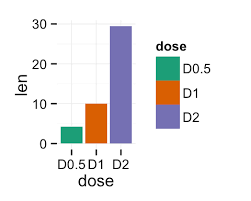
\includegraphics{barplot.png}

}

\end{figure}

Lets take barplots as examples. There are two types of bar charts:
\textbf{\texttt{geom\_bar()}} and \textbf{\texttt{geom\_col()}}.
\textbf{\texttt{geom\_bar()}} makes the height of the bar proportional
to the number of cases in each group (or if the \texttt{weight}
aesthetic is supplied, the sum of the weights). If you want the heights
of the bars to represent values in the data, use
\textbf{\texttt{geom\_col()}} instead.

\uline{Scale functions}

There are different functions to represent the scales of the data in the
plots using R. Those functions can be applied to the x or y axis. The
most common type of scales are:
\textbf{\texttt{scale\_x\_continuous()}},
\textbf{\texttt{scale\_y\_continuous()}},
\textbf{\texttt{scale\_x\_discrete()}},
\textbf{\texttt{scale\_y\_discrete()}},
\textbf{\texttt{scale\_x\_log10()}},
\textbf{\texttt{scale\_y\_log10()}}.

The function \textbf{\texttt{scale\_y\_continuous()}} can be use to
format the y-axis of a continuous variable. For example you can
introduce \texttt{breaks} and \texttt{limits}.

\textbf{\texttt{labs()}} Modify axis, legend, and plot labels. Good
labels are critical for making your plots accessible to a wider
audience. Always ensure the axis and legend labels display the full
variable name. Use the plot \texttt{title} and \texttt{subtitle} to
explain the main findings. It's common to use the \texttt{caption} to
provide information about the data source. \texttt{tag} can be used for
adding identification tags to differentiate between multiple plots.

\uline{Themes}

\textbf{\texttt{theme()}} is a powerful way to customize the non-data
components of your plots: i.e.~titles, labels, fonts, background,
gridlines, and legends. Themes can be used to give plots a consistent
customized look. ggplot has several pre-build themes like:
\textbf{\texttt{theme\_classic()}} and
\textbf{\texttt{theme\_minimal()}}

Example:

\begin{Shaded}
\begin{Highlighting}[]
\FunctionTok{ggplot}\NormalTok{(}\AttributeTok{data =}\NormalTok{ data\_clean) }\SpecialCharTok{+}
  \FunctionTok{geom\_boxplot}\NormalTok{(}\AttributeTok{x =}\NormalTok{ groups,}
               \AttributeTok{y =}\NormalTok{ abundance) }\SpecialCharTok{+}
  \FunctionTok{scale\_y\_continuous}\NormalTok{(}\AttributeTok{limits =} \FunctionTok{c}\NormalTok{(}\DecValTok{0}\NormalTok{, }\DecValTok{0}\NormalTok{),}
                     \AttributeTok{breaks =} \FunctionTok{seq}\NormalTok{(}\DecValTok{0}\NormalTok{, }\DecValTok{100}\NormalTok{, }\DecValTok{10}\NormalTok{)) }\SpecialCharTok{+}
  \FunctionTok{labs}\NormalTok{(}\AttributeTok{y =} \StringTok{"Relative abundance (\%)"}\NormalTok{,}
       \AttributeTok{x =} \StringTok{"Treatment"}\NormalTok{) }\SpecialCharTok{+}
  \FunctionTok{theme\_classic}\NormalTok{()}
\end{Highlighting}
\end{Shaded}

\hypertarget{tidyverse-functions}{%
\subsection{Tidyverse functions}\label{tidyverse-functions}}

rename()

separate()

select()

inner\_join() left\_join() right\_join()

filter()

pivot\_longer()

pivot\_wider()

group\_by()

summarize()

mutate()



\end{document}
